\documentclass[sn-mathphys,Numbered]{sn-jnl}% Math and Physical Sciences Reference Style

%%%% Standard Packages
\usepackage{graphicx}%
\usepackage{amsmath,amssymb,amsfonts}%
\usepackage{xcolor}%
\usepackage{manyfoot}%
\usepackage{booktabs}%
\usepackage{tabularx}%
\usepackage{enumitem}%
\usepackage{tikz}%

% Redpine brand palette (see brand brief) -- the only 7 colours allowed to ship
% under the Redpine name. Never introduce off-palette hues elsewhere in this doc.
\definecolor{RPDarkRed}{HTML}{BD0519}
\definecolor{RPCrimson}{HTML}{EB301F}
\definecolor{RPOrange}{HTML}{FB8520}
\definecolor{RPWarmWhite}{HTML}{FDFBF7}
\definecolor{RPDarkGrey}{HTML}{171717}
\definecolor{RPLightGreen}{HTML}{628F6B}
\definecolor{RPSkyBlue}{HTML}{8BBCE5}

\raggedbottom

\newcommand{\lead}[1]{\textbf{#1}}   % bold run-in lead phrase, e.g. "Method."

% Placeholder box for a chart/graph not yet embedded -- swap for
% \includegraphics once the real image is uploaded to the Overleaf project.
\newcommand{\graphplaceholder}[1]{%
  \begin{center}
  \fbox{\parbox{0.85\linewidth}{\centering\vspace{1.2em}\itshape #1\vspace{1.2em}}}
  \end{center}
}

%own commands and packets 
\usepackage{duckuments}


\newcommand{\todo}[1]{{\color{red}\bf [TODO: #1]}}

\begin{document}

\title[Evaluating Redpine Science]{Leveraging a four tiered approach for evaluating
Redpine Science}

\author[1]{\fnm{Leonora} \sur{Vesterbacka}}

\author[1]{\fnm{Filip} \sur{Dorm}}

\affil[1]{\orgname{Redpine}, \orgaddress{\country{Sweden}}}

\abstract{Redpine Science gives models and agents a single access point to peer-reviewed
literature from seven publishers, queried directly through MCP and API. This report
evaluates Redpine Science along two independent axes: the source of the evaluation
questions (an existing public benchmark, or a literature-grounded question set built
and validated in-house) and what is measured (a full agentic answer, or retrieval
alone, with no model reasoning involved). Crossing these axes gives four separate
evaluations rather than one blended score. An agent with Redpine Science access scores
[X] percentage points higher than an agent restricted to web search on our
expert-validated question set. On document retrieval, stripped of any model reasoning,
Redpine Science recovers the correct source paper 88.9\% of the time, against 61.5\%
for Exa, the retrieval benchmark's own creator, run under its published configuration.
On public answer-quality benchmarks, Redpine Science leads on five of six benchmarks
tested and ties on the sixth, with no losses. A blinded expert relevance panel,
following Consensus's published methodology, places Redpine Science's Precision@5 at
58.9\% against 32.6\% for PubMed.}

\keywords{Evaluation Benchmarks, LLM, RAG}

\maketitle

\section{Introduction}\label{sec:introduction}

Redpine Science gives models and agents a single access point to peer-reviewed
literature from seven publishers, queried directly through MCP~\cite{mcp} and API. This
report measures how much that access improves the answers a model produces, and how
reliably that improvement can be measured.

Evaluating a retrieval-augmented system is harder than evaluating a model alone. A RAG
pipeline conflates two effects: whether the right passage is surfaced (retrieval), and
whether the model turns that passage into an accurate, grounded answer (generation).
Most published evaluations, including ours until recently, report a single blended
score for both. A win on that score can come from better retrieval, a better-written
answer drawn from similar evidence, or some mix of the two, and the number alone does
not distinguish between them.

We separate the two effects by crossing two independent choices: who wrote the
evaluation questions, an existing public benchmark or a literature-grounded set we
built ourselves, and what is measured, the full agentic answer or retrieval alone with
no model reasoning in the loop. This produces four evaluations rather than one,
described in Sections~\ref{sec:method-quadrant-one} through \ref{sec:method-quadrant-four}. Reporting
all four separately lets a result be attributed to retrieval or to generation
specifically.

Questions built by the evaluator carry a specific risk: if they are grounded in content
only the evaluator's own system can access, that system wins by construction, not by
retrieval or reasoning quality. Section~\ref{sec:methodology} describes the
question-generation approach built to avoid that.

\section{Redpine Science}\label{sec:redpine-science}

Redpine Science is built on partnerships with seven publishers, Harvard Business
Publishing, BMJ, Wiley, Sage, Wanfang Data, IGI Global, and IOP, covering clinical
medicine, life sciences, physics, and social sciences. Combined with 50+ existing
partners, this gives models and agents live access to over 20 million peer-reviewed
articles through Redpine's API and MCP.

Corpus breadth is only half the system. The retrieval stack built on top of it, which
embedding model represents a query and a passage, which reranker re-scores the
shortlist before an agent sees it, and how often either is replaced, is maintained
continuously rather than fixed at launch. The results in this report measure that stack
as much as the underlying corpus.

\section{Evaluation methodology}\label{sec:methodology}

Figure~\ref{fig:methodology} shows the four evaluations produced by crossing question
source against what is measured.

\begin{figure}[h]
\centering
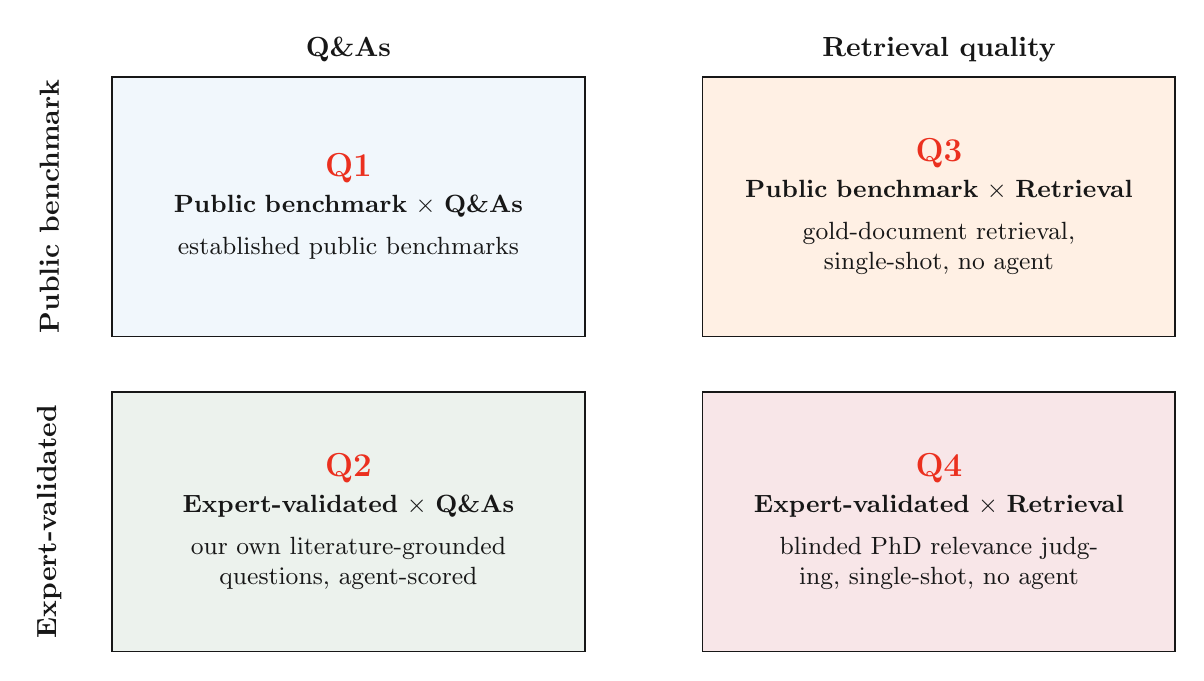
\begin{tikzpicture}[
  quad/.style={draw=RPDarkGrey, line width=0.6pt, text width=5.3cm,
    minimum height=3.3cm, align=center, inner sep=10pt, font=\small, text=RPDarkGrey},
  axis/.style={font=\bfseries, text=RPDarkGrey},
]
  \node[quad, fill=RPSkyBlue!12] (q1) at (0,0)
    {{\bfseries\large\color{RPCrimson}Q1}\\[2pt]
     \textbf{Public benchmark $\times$ Q\&As}\\[4pt]
     established public benchmarks};
  \node[quad, fill=RPOrange!12] (q3) at (7.5,0)
    {{\bfseries\large\color{RPCrimson}Q3}\\[2pt]
     \textbf{Public benchmark $\times$ Retrieval}\\[4pt]
     gold-document retrieval, single-shot, no agent};
  \node[quad, fill=RPLightGreen!12] (q2) at (0,-4)
    {{\bfseries\large\color{RPCrimson}Q2}\\[2pt]
     \textbf{Expert-validated $\times$ Q\&As}\\[4pt]
     our own literature-grounded questions, agent-scored};
  \node[quad, fill=RPDarkRed!10] (q4) at (7.5,-4)
    {{\bfseries\large\color{RPCrimson}Q4}\\[2pt]
     \textbf{Expert-validated $\times$ Retrieval}\\[4pt]
     blinded PhD relevance judging, single-shot, no agent};

  \node[axis] at (0,2.0) {Q\&As};
  \node[axis] at (7.5,2.0) {Retrieval quality};
  \node[axis, rotate=90] at (-3.8,0) {Public benchmark};
  \node[axis, rotate=90] at (-3.8,-4) {Expert-validated};
\end{tikzpicture}
\caption{The four evaluations, crossing question source against measurement target.}
\label{fig:methodology}
\end{figure}

Each cell exists elsewhere in the field individually. Scoring an agent's answer against
public benchmarks or against harder expert-authored questions is standard for RAG and
agent evaluations. Retrieval measured in isolation is also established: search
providers publish benchmark retrieval results for their own products, and blinded human
relevance judging is a recognized method independent of this report. Reporting all four
together, so a retrieval effect and a generation effect can be separated for both
question sources, is this methodology's contribution.

Questions grounded in content only the evaluator's system can access favor that system
by construction, not by retrieval or reasoning quality. Section~\ref{sec:method-quadrant-two}
describes the question-generation approach used to avoid that: domain experts validate
every question before it enters the evaluation set.

\section{Method}\label{sec:method}

\subsection{Quadrant one: public benchmarks, Q\&As}\label{sec:method-quadrant-one}

Public benchmarks let LLM capabilities be evaluated systematically and compared across
labs \todo{add citations}, and biomedicine has a growing set of them. Many are also
likely present in the training data of the models being evaluated, so a high score can
reflect memorization rather than retrieval, integration, and reasoning over new
information. Harder, newer benchmarks correct for this as models improve; on those,
retrieval can still add a measurable benefit, and results stay comparable against other
groups' published numbers.

We run a broad set of biomedical benchmarks spanning this range of difficulty and
memorization risk. Some are already close to saturated, with current models answering
most questions correctly without any retrieval \todo{point to benchmarks}; others are
hard enough that added biomedical information still helps. Running both lets us measure
Redpine retrieval's value in each regime: whether it adds gains where models are already
strong, and whether those gains grow on benchmarks where the relevant information is
hard to access from model parameters alone.


We have six running so far: MedHELM~\cite{medhelm}, MMLU-Redux Biology~\cite{mmluredux},
BioASQ factoid~\cite{bioasq}, BioASQ yes/no~\cite{bioasq}, SciFact fact
verification~\cite{scifact}, and MedXpertQA~\cite{medxpertqa}. HealthBench~\cite{healthbench},
LiveMedBench~\cite{livemedbench}, and Humanity's Last Exam's~\cite{hle} Bio/Chem Gold
subset are still being added.

\subsection{Quadrant two: expert-validated questions, Q\&As}\label{sec:method-quadrant-two}

Public benchmarks are comparable across labs, but a model that has
memorized the answer is not testing retrieval. We built a harder question set grounded
in the literature Redpine Science covers: each question is built through reasoning
steps that narrow and constrain the answer, and is answerable only from a source
paper's full text, not its freely available abstract. \todo{add more details on what models and such we use}

Every generated question is reviewed by PhD-level experts in the relevant field before
entering the evaluation set, removing ambiguous, trivially answerable, or incorrect
questions before they can distort a result. \todo{for this we built an annotation tool where the experts were asked to assess the quality of different questions, reject them and modify them. the initial llm generating pipeline produced questions of quality split X good/Y needs edit / Z bad}.

\lead{Experimental setup.} Two near-identical setups, differing only in the tools they
have access to, run on identical prompts: an agent with access to
both Redpine Science and web search (via Tavily \todo{add source}), against an agent with web search
only, isolating the value Redpine adds on top of an agent's existing capabilities.
Model, system prompt, and step budget are held constant between arms; only tool access
to Redpine's retrieval varies.

\lead{Judging setup and criteria.} Every answer is scored by a fixed LLM judge, held
constant across both arms and distinct from the model producing the answer. Four
criteria make up the final answer score:

\begin{itemize}[leftmargin=1.6em, itemsep=0.3em]
  \item \textbf{Correctness.} Does the answer contradict anything the gold rubric says?
  \item \textbf{Completeness.} Does the answer cover every part of what was asked?
  \item \textbf{Directness.} Does the answer commit to a clear conclusion, or hedge?
  \item \textbf{Source quality.} How authoritative are the sources the answer draws on?
\end{itemize}

\[
  \text{Overall} = \frac{\text{Correctness} + \text{Completeness} + \text{Directness}
  + \text{Source quality}}{4}
\]

Faithfulness, whether each claim is grounded in the raw retrieved text, is scored
separately from Overall: it is near-constant across both arms in our runs, showing both
are equally grounded but not distinguishing which arm is better. Two further criteria,
adapted from the RAGAS evaluation framework~\cite{ragas} and computed with
DeepEval~\cite{deepeval}, score retrieval directly, separate from the answer score,
distinguishing a weak final answer built on strong retrieval from one built on weak
retrieval:

\begin{itemize}[leftmargin=1.6em, itemsep=0.3em]
  \item \textbf{Contextual recall.} Does the retrieved context contain everything
    needed to support the gold answer? Sentences supported by retrieved context
    divided by total sentences.
  \item \textbf{Contextual relevancy.} How much of what got retrieved was actually
    useful? Retrieved statements judged relevant divided by total retrieved
    statements.
\end{itemize}

\lead{Evaluation dataset.} 53 questions so far, over seven fields: oncology, public
health, neurology, pharmacology, psychiatry, cardiovascular disease, and infectious
disease, full text only.

\subsection{Quadrant three: public benchmarks, retrieval quality}\label{sec:method-quadrant-three}

Quadrants one and two score the full agentic answer, where a poor result
may reflect generation rather than retrieval, and a strong result may reflect writing
quality compensating for weak retrieval. Quadrant three isolates retrieval directly:
one query in, one ranked list out, no agent loop, no reformulation, no reasoning. Each
system answers with only its own ranking, once.

We used an existing open benchmark rather than building our own: a self-built one is
the easiest place to rig a result, pick your own gold documents and any retriever
indexed on them wins.

The Exa publication-retrieval benchmark~\cite{exabenchmarks} grounds every query in one
gold publication and scores whether it was surfaced, by DOI or title, at what rank. It
asks several phrasings per source paper, so its 351 DOI-confirmed queries map to 55
unique source papers. We report recall at the query level, the more demanding number,
since it counts every phrasing separately. We restrict to these 351 queries rather than
the benchmark's full 1,866: the rest ask about papers outside Redpine's corpus, and
scoring Redpine on documents it cannot hold would measure corpus coverage rather than
retrieval quality. We ran two retrieval services against it, queried
identically, no follow-up fetch, no agent reasoning: Redpine Science, and Exa's own
search, run the way exa-labs/benchmarks' own GitHub repository describes running it.
Neither is a web agent. Both are retrieval services, Exa over the open web, Redpine
Science over a curated, licensed corpus, so this compares retrieval quality on
identical terms.

Exa is included because it is this benchmark's own creator: beating the engine that
built and calibrates itself against this exact benchmark, run the way its own team runs
it, is a harder result to dismiss than beating an unrelated product.

\subsection{Quadrant four: expert-validated questions, retrieval quality}\label{sec:method-quadrant-four}

Quadrant three measures whether a system finds one known document. It
says nothing about relevance for the kind of open, comparative question a domain expert
actually asks, where multiple passages may be defensible and judging which is better is
not a lookup. That judgment requires a human expert, blinded to which system produced
each result.

Judges score each result on a 0 to 4 scale, 0 not relevant, 4 perfectly relevant,
matching the scale and Precision@K / DCG@K reporting used by Consensus's own relevance
evaluation~\cite{consensus}, blind to which system produced it; system identity is
randomized left-to-right per query to prevent a judge from guessing rather than
reading. Every result is stripped of anything that would give the system away before a
judge reads it: URL, DOI, and publication date are all removed, since a database record
and a scraped web page format these differently enough to identify the source on their
own.

The comparison arm is PubMed: what a researcher actually types a question into today,
not the most sophisticated retrieval competitor available. Both arms receive the
identical, unmodified question text, with no query engineering on either side.

Two PhD-level domain experts are the judges. One judge's 30 questions are mostly
neurology, with a handful of adjacent critical care, immunology, microbiology, and
pharmacology questions; the other's 30 are entirely cardiology: hard subspecialty
questions that require real domain knowledge to even evaluate the results, not just to
answer. Each judge scores the top 5 results per system for their own batch. The two
batches do not overlap, so every number below pools both judges' ratings rather than
measuring inter-rater agreement on shared queries.

\section{Results}\label{sec:results}

\subsection{Quadrant one: public benchmarks, Q\&As}\label{sec:results-quadrant-one}

\begin{figure}[htbp]
    \centering
    \includegraphics[width=0.5\textwidth]{example-image-duck}
    \caption{Graph: per-benchmark comparison, web search vs.\ Redpine}
    \label{fig:duck_placeholder}
\end{figure}

Redpine Science leads on five of six benchmarks and ties on the sixth,
MedXpertQA, with no losses. Only one win clears conventional significance: BioASQ
factoid, at $p = 0.017$, run on 127 questions against 15 to 24 for the rest. The
remaining wins, MedHELM (+20.8 points), MMLU-Redux Biology (+13.3), BioASQ yes/no
(+8.3), and SciFact (+8.3), are directional but not individually significant at this
sample size; more queries are needed before treating any one of them as more than
consistent with a real effect.

\subsection{Quadrant two: expert-validated questions, Q\&As}\label{sec:results-quadrant-two}

\begin{figure}[htbp]
    \centering
    \includegraphics[width=0.5\textwidth]{example-image-duck}
    \caption{Preliminary per-criterion comparison, Connect vs.\ web search, n=57,
95\% CI error bars, margin and paired p-value under each pair}
    \label{fig:duck_placeholder}
\end{figure}

\subsection{Quadrant three: public benchmarks, retrieval quality}\label{sec:results-quadrant-three}

\begin{table}[h]
\caption{Quadrant three retrieval results, n=351.}
\label{tab:quadrant-three}
\begin{tabular}{@{}lccc@{}}
\toprule
 & \textbf{Recall} & \textbf{MRR} & \textbf{nDCG} \\
\midrule
Redpine Science & 88.9\% & 0.769 & 0.798 \\
Exa             & 61.5\% & 0.442 & 0.484 \\
\bottomrule
\end{tabular}
\end{table}

Redpine leads clearly, and when it surfaces the right paper at all, it is
disproportionately at rank one. We followed exa-labs/benchmarks' own setup for Exa.

We are grateful to Exa for publishing this benchmark openly; this quadrant would not
exist without it.

\subsection{Quadrant four: expert-validated questions, retrieval quality}\label{sec:results-quadrant-four}

\begin{figure}[htbp]
    \centering
    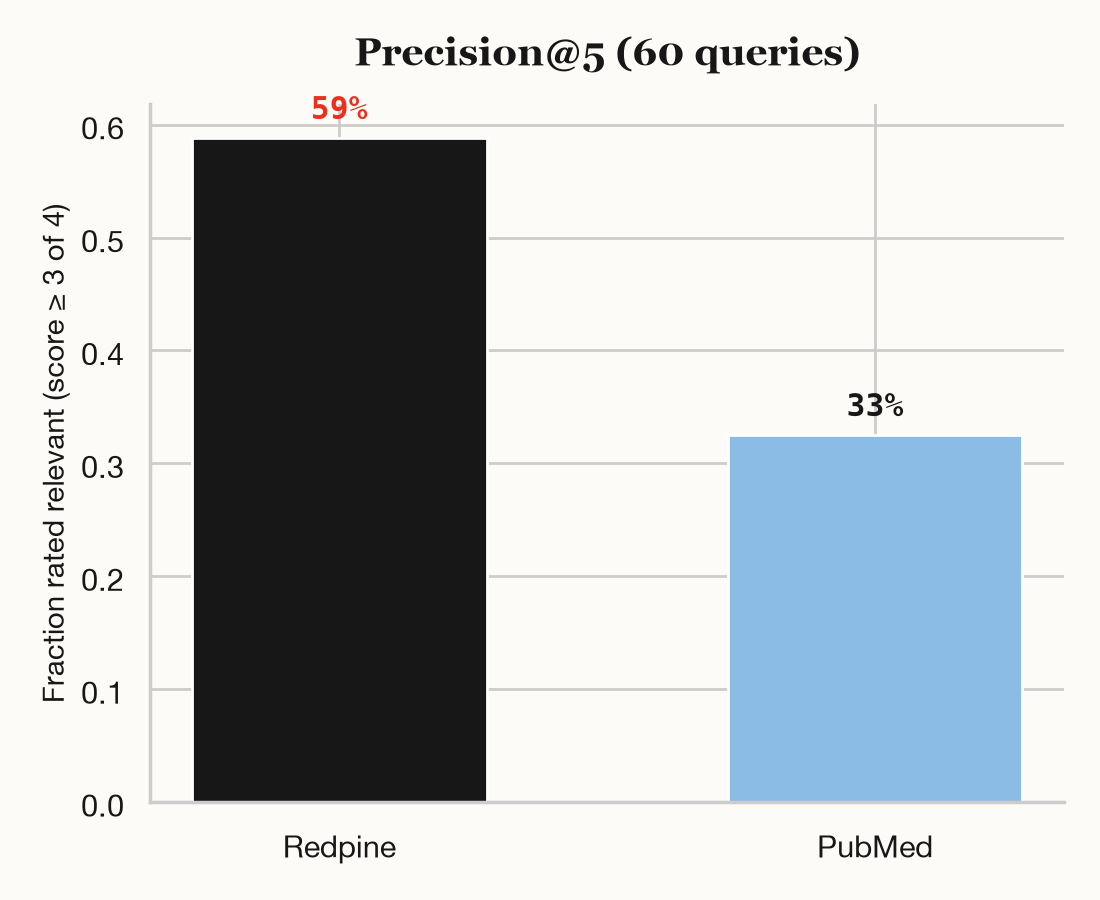
\includegraphics[width=0.7\textwidth]{figures/quadrant4_precision_at_5.png}
    \caption{Precision@5, fraction of results scored 3 or 4 of 4, by system, pooled
    across both judges (n=60 queries).}
    \label{fig:quadrant4-precision}
\end{figure}

\begin{figure}[htbp]
    \centering
    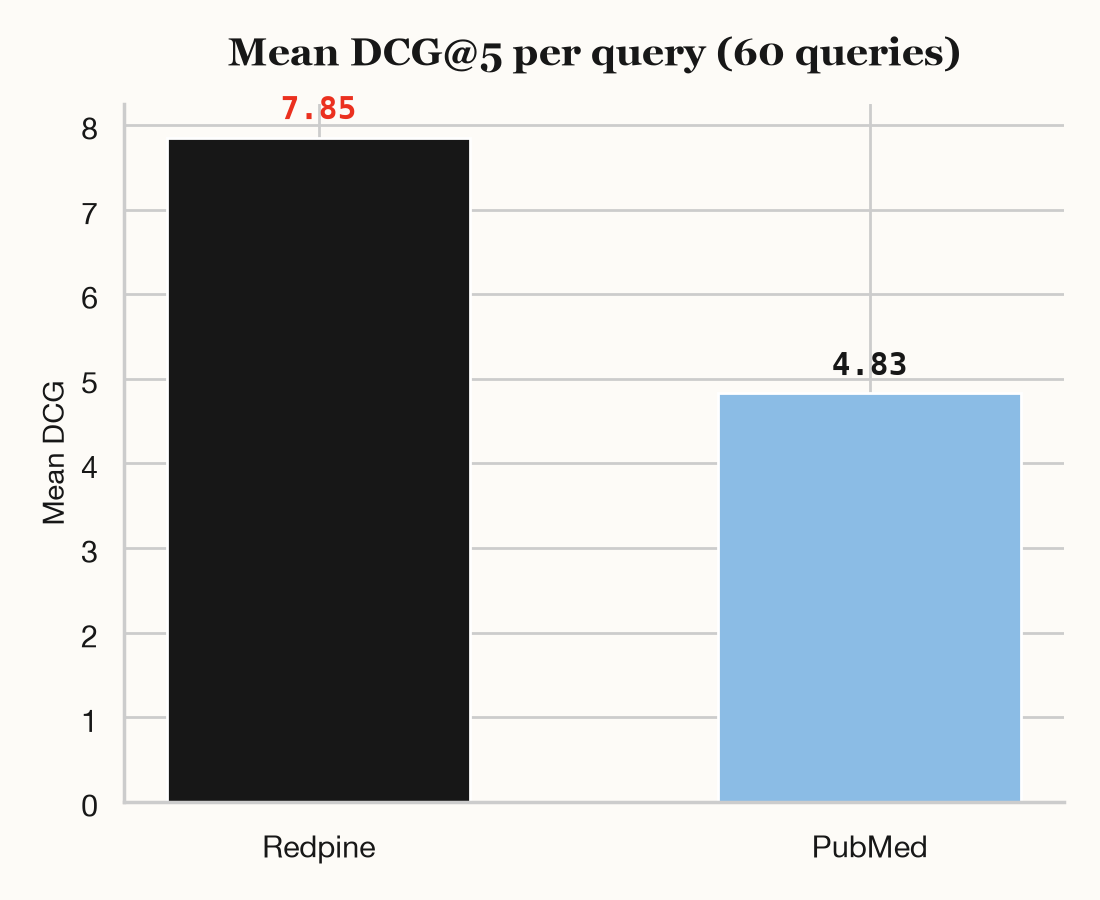
\includegraphics[width=0.7\textwidth]{figures/quadrant4_dcg_at_5.png}
    \caption{Mean DCG@5 per query, by system, pooled across both judges (n=60
    queries).}
    \label{fig:quadrant4-dcg}
\end{figure}

Redpine Science leads on both metrics: Precision@5 58.9\% against 32.6\% for PubMed,
mean DCG@5 7.85 against 4.83. Mean relevance per judged result is 2.64 against 1.66 on
the 0 to 4 scale. The margin holds in the same direction for both judges individually:
the mostly-neurology batch scores Redpine Science at 49.0\% Precision@5 against 20.8\%
for PubMed; the cardiology batch scores 68.7\% against 44.3\%.


\section{What we are releasing}\label{sec:releasing}

Alongside these results, we are open-sourcing the expert-validated question set and the
agentic evaluation harness used to produce the answer-quality results above.

\begin{itemize}[leftmargin=1.6em, itemsep=0.5em]
  \item \textbf{The expert-validated question set.} The depth questions, gold rubrics
    included, at [link to GitHub repository].
  \item \textbf{An evaluation harness.} The agentic evaluation framework used for the
    answer-quality quadrants, comparing an agent with and without access to Redpine
    Science.
\end{itemize}

\section{Summary}\label{sec:summary}

On our expert-validated question set, an agent with Redpine Science access scores [X]
percentage points higher than an agent restricted to web search. On the public
retrieval benchmark, Redpine Science recovers the correct document 88.9\% of the time,
against 61.5\% for Exa, the benchmark's own creator. On the expert-judged retrieval
panel, two PhD-level domain experts (neurology and cardiology) place Redpine Science's
Precision@5 at 58.9\% against 32.6\% for PubMed; a scaled-up expert-validated answer
set will be reported ahead of launch.

\section{Acknowledgments}\label{sec:thanks}

Quadrant three depends directly on Exa's decision to publish its
publication-retrieval benchmark~\cite{exabenchmarks} openly. Quadrant one depends
similarly on MMLU-Redux~\cite{mmluredux}, MedXpertQA~\cite{medxpertqa},
HealthBench~\cite{healthbench}, LiveMedBench~\cite{livemedbench},
MedHELM~\cite{medhelm}, BioASQ~\cite{bioasq}, and Humanity's Last Exam~\cite{hle}, each
built and released publicly by its creators; every comparison in this report against
other labs' results is possible because of that choice. Evaluation infrastructure of
this kind is a shared resource.
\todo{thank our phd evaluators, felix perhaps}

\begin{thebibliography}{99}

\bibitem{mcp}
Anthropic.
\newblock Introducing the Model Context Protocol.
\newblock Anthropic News, November 2024.
  \url{https://www.anthropic.com/news/model-context-protocol}

\bibitem{medhelm}
S.~Bedi, H.~Cui, M.~Fuentes, A.~Unell, M.~Wornow, et~al.
\newblock MedHELM: Holistic Evaluation of Large Language Models for Medical
  Tasks.
\newblock \emph{arXiv preprint arXiv:2505.23802}, 2025.

\bibitem{mmluredux}
A.~P. Gema, J.~O.~J. Leang, G.~Hong, A.~Devoto, A.~C.~M. Mancino, et~al.
\newblock Are We Done with MMLU?
\newblock \emph{arXiv preprint arXiv:2406.04127}, 2024.

\bibitem{bioasq}
G.~Tsatsaronis, G.~Balikas, P.~Malakasiotis, I.~Partalas, M.~Zschunke, et~al.
\newblock An overview of the BIOASQ large-scale biomedical semantic indexing
  and question answering competition.
\newblock \emph{BMC Bioinformatics}, 16:138, 2015.
  \url{https://doi.org/10.1186/s12859-015-0564-6}

\bibitem{scifact}
D.~Wadden, S.~Lin, K.~Lo, L.~L. Wang, M.~van Zuylen, A.~Cohan, and
  H.~Hajishirzi.
\newblock Fact or Fiction: Verifying Scientific Claims.
\newblock In \emph{Proceedings of the 2020 Conference on Empirical Methods in
  Natural Language Processing (EMNLP)}, pages 7534--7550, 2020.

\bibitem{medxpertqa}
Y.~Zuo, S.~Qu, Y.~Li, Z.~Chen, X.~Zhu, E.~Hua, K.~Zhang, N.~Ding, and
  B.~Zhou.
\newblock MedXpertQA: Benchmarking Expert-Level Medical Reasoning and
  Understanding.
\newblock \emph{arXiv preprint arXiv:2501.18362}, 2025. ICML 2025.

\bibitem{healthbench}
R.~K. Arora, J.~Wei, R.~S. Hicks, P.~Bowman, et~al.
\newblock HealthBench: Evaluating Large Language Models Towards Improved
  Human Health.
\newblock \emph{arXiv preprint arXiv:2505.08775}, 2025.

\bibitem{livemedbench}
Z.~Yan, D.~Song, Z.~Fang, Y.~Ji, X.~Li, Q.~Li, and L.~Sun.
\newblock LiveMedBench: A Contamination-Free Medical Benchmark for LLMs with
  Automated Rubric Evaluation.
\newblock \emph{arXiv preprint arXiv:2602.10367}, 2026.

\bibitem{hle}
L.~Phan, A.~Gatti, Z.~Han, N.~Li, J.~Hu, H.~Zhang, et~al.
\newblock Humanity's Last Exam.
\newblock \emph{Nature}, 2025/2026. \url{https://doi.org/10.1038/s41586-025-09962-4};
  preprint \emph{arXiv:2501.14249}.

\bibitem{ragas}
S.~Es, J.~James, L.~Espinosa Anke, and S.~Schockaert.
\newblock Ragas: Automated Evaluation of Retrieval Augmented Generation.
\newblock In \emph{Proceedings of the 18th Conference of the European
  Chapter of the Association for Computational Linguistics: System
  Demonstrations}, pages 150--158, 2024.

\bibitem{deepeval}
Confident AI.
\newblock confident-ai/deepeval: The LLM Evaluation Framework.
\newblock GitHub repository. \url{https://github.com/confident-ai/deepeval}

\bibitem{exabenchmarks}
Exa Labs.
\newblock exa-labs/benchmarks: Open benchmarks for evaluating search APIs.
\newblock GitHub repository, 2026.
  \url{https://github.com/exa-labs/benchmarks}

\bibitem{consensus}
Consensus.
\newblock Consensus Outperforms Google Scholar for Academic Search Retrieval.
\newblock Consensus blog, 2025.
  \url{https://consensus.app/home/blog/consensus-outperforms-google-scholar-for-academic-search-retrieval/}

\end{thebibliography}

\end{document}
